\documentclass[12pt,a4paper]{report}
\linespread{1.3}
\usepackage[utf8]{inputenc}
\usepackage{polski}
\usepackage{graphics}
\usepackage{changepage}
\usepackage{caption}
\usepackage{subcaption}
\usepackage{float}
\usepackage{url}
\usepackage[all]{xy}
\usepackage{tikz}
\usepackage{algorithm}
\usepackage{algpseudocode}
\usepackage{bchart}
\usepackage{colortbl}
\usepackage{hhline}
\usepackage{soul}
\usepackage{forest}
\usepackage[perpage]{footmisc}
\usetikzlibrary{arrows}

\makeatletter
\renewcommand{\ALG@name}{Algorytm}
\makeatother
\newcommand{\source}[1]{\caption*{\textbf{Źródło}: {#1}} }		

\begin{document}
	\author{Aleksander Krzeszowski}
	\title{Aplikacja usprawniająca pracę kuriera -- problem komiwojażera w praktyce}
	
	\begin{titlepage}
	\begin{adjustwidth*}{-2cm}{-2cm}
		\centering
	
\includegraphics[width=0.5\textwidth]{pk.png}\par
	\vspace{0.5cm}
	{\scshape Wydział Inżynierii Elektrycznej i~Komputerowej\par}
	\vspace{2cm}
	
	{\huge\bfseries Aplikacja usprawniająca pracę kuriera -- problem komiwojażera w praktyce\par}
	
	\vspace{0.5cm}
	{\Large Aleksander Krzeszowski\par}
	\vfill
	Promotor:\par
	dr inż. Damian \textsc{Grela}
	\vfill

% Bottom of the page
	{\large Kraków, \today\par}
	\end{adjustwidth*}
\end{titlepage}
		
	\tableofcontents
	\addtocontents{toc}{\protect\enlargethispage{3\baselineskip}}	
	\chapter*{Wstęp}
		\addcontentsline{toc}{chapter}{Wstęp}
		Wprowadzenie.
	\chapter{Definicja i rozwiązanie problemu}
		\label{ch:definicja_i_rozwiazanie}
		\section{Określenie problemu}
			Problem komiwojażera polega na wyznaczeniu trasy łączącej wybrane punkty\footnote{Pierwotnie problem dotyczył tras między miastami, przez co w opracowaniach lub algorytmach punkty pośrednie często nazywa się miastami}, przy dodatkowych warunkach: każdy punkt może zostać odwiedzony wyłącznie raz, poza wybranym punktem będącym początkiem i końcem trasy. Można więc powiedzieć, że rozwiązanie stanowi permutacja $n$ punktów, a~optymalnym rozwiązaniem jest permutacja o minimalnej sumie odległości między punktami\cite{genetyczne}.

\begin{figure}[h!]
	\begin{displaymath}
	\xygraph{
		!{<0cm,0cm>;<1.5cm,0cm>:<0cm,1.2cm>::}
		!{(0,0) }*+{\bullet_{A}}="a"
		!{(1,1) }*+{\bullet_{B}}="b"
		!{(2.5,0.5) }*+{\bullet_{C}}="c"
		!{(2,-1)}*+{\bullet_{D}}="d"
		"a"-"b" ^3
		"a"-"c" ^(0.4)4
		"a"-@/_/"d" ^2
		"b"-"c" ^9
		"b"-@/_/"d" ^(0.6){13} 
		"c"-"d" ^1
	}
\end{displaymath}
\caption{Przykład symetryczny: Reprezentacja grafowa}
\label{fig:przyklad1_komiwojazer_graf}
\end{figure}
Przykładowy problem został przedstawiony na grafie \ref{fig:przyklad1_komiwojazer_graf}. Przyjmując $B$ za punkt startowy, optymalną trasą dla takiego zbioru punktów jest na przykład: $B \to A \to D \to C \to B$ o~długości 15.

Punkty pośrednie stanowią wierzchołki grafu, a trasy je łączące to krawędzie o wagach równych odległościom między punktami. Powyższy prosty przykład to wariant symetryczny problemu komiwojażera -- odległości między dwoma punktami są identyczne w każdym kierunku. Dla takiego grafu wystarczy odnaleźć wagi dla $\frac{n(n-1)}{2}$ krawędzi, ponieważ są nieskierowane.

\begin{table}
	\begin{center}
		\begin{tabular}
			{  c | c c c c }
			& A & B & C & D \\
			\hline
			A & 0 & 3 & 4 & 2 \\
			B & 3 & 0 & 9 &13 \\
			C & 4 & 9 & 0 & 1 \\
			D & 2 &13 & 1 & 0 \\
		\end{tabular}
	\end{center}
	\caption{Przykład symetryczny: Macierz sąsiedztwa}
	\source{Opracowanie własne}
\end{table}

Jednak w rzeczywistym zastosowaniu (a także w zrealizowanej aplikacji) mamy do czynienia z asymetryczną wersją problemu, a więc ze skierowanym grafem. Jest to spowodowane tym, że co prawda z dowolnego punktu możemy dotrzeć do innego, jednak trasy między dwoma punktami mogą być inne (na przykład ulice jednokierunkowe). W rezultacie konieczne jest odnalezienie $n^2-n$ odległości między punktami.
\begin{figure}[t!]
	\centering
	\def\svgwidth{0.6\columnwidth}
	\input{asymetryczny.pdf_tex}
	\caption{Przykład asymetryczny: Reprezentacja grafowa}
	\label{fig:przyklad2_komiwojazer_graf}
\end{figure}

\begin{table}[H]
	\begin{center}
		\begin{tabular}
			{  c | c c c c }
			& A & B & C & D \\
			\hline
			A & 0  & 13 & 9  &  7 \\
			B & 2  & 0  & 8  &  8 \\
			C & 13 & 14 & 0  &  3 \\
			D & 12 & 2  & 24 &  0 \\
		\end{tabular}
	\end{center}
	\caption{Przykład symetryczny: Macierz sąsiedztwa}
	\source{Opracowanie własne}
\end{table}

Przykład problemu asymetrycznego znajduje się na grafie \ref{fig:przyklad2_komiwojazer_graf}. Najkrótszą trasą rozpoczynającą się w punkcie $C$ jest $C \to D \to B \to A \to C$ o~długości~16.

Warto zauważyć że dla algorytmów nie ma znaczenia w jakiej jednostce jest wyrażona waga -- można więc tym samym algorytmem optymalizować zarówno odległość, jak i czas przejazdu.

\clearpage
		\section{Algorytmy genetyczne}
			Ogólny przebieg algorytmu ewolucyjnego wygląda następująco:

\begin{algorithm}
	\caption{Program ewolucyjny\hfill\textbf{Źródło}: \cite{genetyczne} }\label{ewolucyjny}
	\begin{algorithmic}[1]
		\Procedure{Program Ewolucyjny}{}
		\State $t\gets 0$
		\State ustal początkowe $P(t)$ 	\Comment Inicjalizacja
		\While{\textbf{not} warunek zakończenia}
			\State $t\gets t + 1$
			\State wybierz $P(t)$ z $P(t - 1)$ \Comment Selekcja
			\State zmień $P(t)$ \Comment Krzyżowanie i mutacja
			\State oceń $P(t)$ \Comment Funkcja oceny
		\EndWhile
		\EndProcedure
	\end{algorithmic}
\end{algorithm}

W kolejnych podrozdziałach zostaną omówione poszczególne etapy programu.
		\subsection{Inicjalizacja}
			Inicjalizacja polega na wygenerowaniu populacji złożonej z losowych osobników. W~przypadku problemu komiwojażera populację stanowi zbiór tras, składających się z~punktów pośrednich, dlatego należy spełnić warunek, że każdy element musi wystąpić dokładnie raz w wylosowanej trasie.

Najprostszym sposobem na spełnienie powyższego warunku jest przetasowanie zbioru wszystkich punktów. Opracowany program korzysta ze współczesnej wersji algorytmu Fishera-Yatesa\cite{shuffle}. Ma on złożoność $O(n)$ względem oryginalnego algorytmu o złożoności $O(n^{2})$. Algorytm polega na wykonaniu $n$~zamian między $n$-tym elementem zbioru, a losowym elementem, gdzie $n$~jest równe liczbie elementów zbioru.

Wybór większego rozmiaru populacji zapewnia większą różnorodność, a~w~rezultacie zwiększa prawdopodobieństwo odnalezienia lepszego rozwiązania. Jednak zwiększanie tego parametru wydłuża czas działania algorytmu, co może być niepożądane przez użytkownika. Dlatego rozmiar populacji jest jednym z parametrów dostępnych do modyfikacji przez użytkownika -- może on samodzielnie dobrać rozmiar odpowiadający wymaganej poprawności i~czasowi przetwarzania.
		\subsection{Funkcja oceny}
			Ocena rozwiązania polega na przypisaniu wartości liczbowej danemu rozwiązaniu, tak aby dało się wybrać bardziej optymalne przy porównywaniu. Dla trasy jest to jej całkowita długość, czyli suma długości odcinków od wybranego punktu, między wszystkimi punktami pośrednimi i od ostatniego punktu pośredniego do punktu początkowego.

Punkty są przechowywane w aplikacji w postaci grafowej, więc odnalezienie długości trasy jest proste. Wszystkie punkty zawiera zbiór odległości do każdego innego punktu. Odległości są przechowywane we standardowej kolekcji \texttt{Dictionary<T>}, która jest zaimplementowana w postaci tablicy z~haszowaniem, umożliwiającej odnalezienie elementu w średnim czasie $O(1)$. Dlatego obliczanie całkowitej odległości ma złożoność bliską liniowej.

Aplikacja umożliwia także wyszukiwanie tras bez określonego punktu początkowego. Przy tej samej liczbie wszystkich punktów skorzystanie z tej opcji zwiększa liczbę możliwych tras, co utrudnia odnalezienie tej najkrótszej. 

Ponieważ kurierzy po dostarczeniu wszystkich przesyłek zazwyczaj nie muszą wracać do sortowni, dodana została również opcja wyłączenia powrotu do punktu początkowego. 
		\subsection{Selekcja}
			Selekcja kandydatów do krzyżowania przebiega metodą turniejową\cite{turniej}. Polega na wybraniu losowych osobników z populacji, a następnie zapisaniu najlepszego (według kryterium funkcji oceny). Identycznie dokonuje się wyboru drugiego osobnika do krzyżowania.

Często turniej przeprowadza się dla dwóch losowych osobników -- wtedy nazywa się turniejem binarnym. Można również użyć tej metody dla większej liczby osobników. Rozmiar turnieju jest konfigurowalny w aplikacji, a domyślnie jest równy 5.

Liczba operacji w selekcji turniejowej jest zależna od rozmiaru turnieju -- złożoność tego algorytmu to $O(n)$.
		\subsection{Krzyżowanie}
			Krzyżowanie to proces łączenia cech dwóch chromosomów, prowadzący do stworzenia potomka przez wymianę odcinków chromosomów rodziców\cite{genetyczne}.

Klasyczne metody krzyżowania używane dla innych problemów, w przypadku problemu komiwojażera okazują się niewydajne. Przy prostym krzyżowaniu (np. dwupunktowym) uzyskany osobnik mógłby zawierać duplikaty, które sprawiają że rozwiązanie jest błędne. Można zlikwidować nieprawidłowe elementy przez dodatkowe ,,naprawianie'', jednak lepszą metodą jest użycie algorytmu wyspecjalizowanego do danego problemu.

Jako metodę krzyżowania w aplikacji został wybrany algorytm OX\footnote{Ordered Crossover} autorstwa L. Davisa\cite{davis1985applying}. Wynikiem krzyżowania tym algorytmem jest poprawna trasa (metoda gwarantuje brak duplikatów), dlatego jest dobrym wyborem do rozwiązywania problemu komiwojażera.

\noindent\textbf{Przykład:}
Dla rodziców $P_{1}$ i $P_{2}$ wybrano dwa losowe punkty: o indeksach 2 i 4 (licząc od zera). Należy przepisać elementy między wybranymi punktami krzyżowania z pierwszego rodzica do potomka, równocześnie usuwając je z~drugiego chromosomu.
\bigskip

\begin{minipage}[t]{0.5\textwidth}
	 \begin{tabular}{r|c|c|c|c|c|c|c|c|}
	 	\hhline{~*{8}{-}}
	 	$P_{1}$: & 1 & 2 & \cellcolor{blue!25}3 & \cellcolor{blue!25}4 & \cellcolor{blue!25}5 & 6 & 7 & 8 \\
	 	
	 	\hhline{~*{8}{=}}
	 	
	 	$P_{2}$: & 3 & 7 & \cellcolor{blue!25}2 & \cellcolor{blue!25}1 & \cellcolor{blue!25}8 & 6 & 4 & 5 \\
	 	\hhline{~*{8}{-}}
	 \end{tabular} 
\end{minipage}
\begin{minipage}[t]{0.5\textwidth}
	 \begin{tabular}{r|c|c|c|c|c|c|c|c|}
	 	\hhline{~*{8}{-}}
	 	$O$: & \hphantom{5} & \hphantom{5} & 3 & 4 & 5 & \hphantom{5} & \hphantom{5} & \hphantom{5} \\
	 	\hhline{~*{8}{-}}
	 \end{tabular} 
\end{minipage}

%\vspace{1cm}
\bigskip
Następnie trzeba wypełnić brakujące indeksy potomka pozostałymi elementami drugiego rodzica zachowując kolejność.
\bigskip

\begin{minipage}[t]{0.5\textwidth}
	\begin{tabular}{r|c|c|c|c|c|c|c|c|}
		\hhline{~*{8}{-}}
		$P_{1}$: & 1 & 2 & \cellcolor{blue!25}3 & \cellcolor{blue!25}4 & \cellcolor{blue!25}5 & 6 & 7 & 8 \\
		
		\hhline{~*{8}{=}}
		
		$P_{2}$: & \st{3} & 7 & \cellcolor{blue!25}2 & \cellcolor{blue!25}1 & \cellcolor{blue!25}8 & 6 & \st{4} & \st{5} \\
		\hhline{~*{8}{-}}
	\end{tabular} 
\end{minipage}
\begin{minipage}[t]{0.5\textwidth}
	\begin{tabular}{r|c|c|c|c|c|c|c|c|}
		\hhline{~*{8}{-}}
		$O$: & 7 & 2 & 3 & 4 & 5 & 1 & 8 & 6 \\
		\hhline{~*{8}{-}}
	\end{tabular} 
\end{minipage}

\begin{center}
	\textbf{Źródło:} Opracowanie własne na podstawie \cite{davis1985applying}
\end{center}

Krzyżowanie zostało zakończone -- potomek $O$ zawiera cechy chromosomów obu rodziców.
		\subsection{Mutacja}
			Mutacja to etap wprowadzania losowych zmian do chromosomu w celu zachowania różnorodności populacji. Pozwala zmniejszyć szanse wystąpienia sytuacji, w której krzyżowanie nadmiernie przystosowanych osobników nie poprawi wyniku w kolejnych pokoleniach.

Podczas mutacji istnieje identyczny problem jak przy etapie krzyżowania -- jej wynikiem musi być poprawna trasa. Prostym sposobem jej przeprowadzenia jest losowanie dwóch punktów, a następnie zamiana ich kolejności. 

\noindent\textbf{Przykład:}
Dla osobnika $O$ wybrano dwa losowe punkty: o indeksach 1 i 5 (licząc od zera). Elementy znajdujące się pod tymi indeksami zostały zamienione w osobniku $M$.

\bigskip

\begin{minipage}[t]{0.5\textwidth}
	\begin{tabular}{r|c|c|c|c|c|c|c|c|}
		\hhline{~*{8}{-}}
		$O$: & 1 & \cellcolor{blue!25}2 & 3 & 4 & 5 & \cellcolor{blue!25}6 & 7 & 8 \\
		\hhline{~*{8}{-}}
	\end{tabular} 
\end{minipage}
\begin{minipage}[t]{0.5\textwidth}
	\begin{tabular}{r|c|c|c|c|c|c|c|c|}
		\hhline{~*{8}{-}}
		$M$: & 1 & 6 & 3 & 4 & 5 & 2 & 7 & 8 \\
		\hhline{~*{8}{-}}
	\end{tabular} 
\end{minipage}

\begin{center}
	\textbf{Źródło:} Opracowanie własne 
\end{center}

O ilości powyższych zamian decyduje współczynnik mutacji - konfigurowalny parametr, określający jak liczna część wszystkich punktów powinna zostać zamieniona. Współczynnik ten nie powinien być zbyt wysoki, gdyż za duża liczba losowych modyfikacji może uszkodzić najlepsze osobniki. Domyślna wartość tego parametru w aplikacji to 0,1.
	\chapter{Implementacja}
		\section{Struktura projektu}
			Aplikacja została zrealizowana w języku C\#. Jest to zorientowany obiektowo język korzystający z .NET Framework \cite{csharp}. Do tworzenia aplikacji w tej technologii można skorzystać z darmowego środowiska Visual Studio. Język ten został wybrany głównie ze względu na możliwość stworzenia w nim aplikacji internetowej w technologii ASP.NET oraz dobrą wydajność pozwalającą na szybkie dokonanie obliczeń. 

C\# jest kompilowany do kodu pośredniego (CIL), przez co jego szybkość jest nieco niższa od języków kompilowanych do języka maszynowego, jak np. C, C++. Jednak skompilowany kod pośredni jest mocno zoptymalizowany, co pozwala na użycie go także w czasochłonnych obliczeniach, a niższa wydajność względem kodu natywnego jest praktycznie niezauważalna.

Praca w Visual Studio polega na stworzeniu \textit{solucji}, czyli zbioru powiązanych projektów tworzących po skompilowaniu gotową aplikację. Podział na projekty umożliwia skorzystanie z różnych języków i kompilatorów w jednej solucji, a także logiczny podział komponentów. Powiązania między projektami są określane przez \textit{referencje}. Po określeniu które projekty są zależne od innych, kompilator potrafi automatycznie ustalić kolejność ich budowania.

Solucja opisywanej aplikacji składa się z trzech projektów:

\subsection*{TSP} 

\begin{figure}
	\centering
	\def\svgwidth{\columnwidth}
	\input{rest.pdf_tex}
	\caption{Schemat komunikacji między serwerem aplikacji oraz potencjalnymi klientami usługi sieciowej}
	\source{Opracowanie własne}
	\label{fig:rest_api}
\end{figure}

Przeglądarkowy interfejs użytkownika, napisany w AngularJS, który korzysta z API\footnote{Application Programming Interface} stworzonego w ASP.NET. API zostało zrealizowane jako \textit{webservice} w konwencji REST\footnote{Representional State Transfer}: udostępnia wszystkie funkcjonalności przy użyciu standardowych metod HTTP, co pozwala łatwo napisać alternatywny interfejs, na przykład w formie aplikacji mobilnej. Schemat komunikacji z API został przedstawiony na rysunku \ref{fig:rest_api}. Klient może pobrać listę punktów pośrednich na mapie, wysyłając żądanie typu \texttt{GET}, lub podając identyfikator punktu wybrać pojedynczy punkt. Zarówno odpowiedzi serwisu jak i~żądania klienta składają się z obiektów zserializowanych do tekstowego formatu JSON\footnote{JavaScript Object Notation}, który stanowi alternatywę dla XML o czytelniejszej składni. Pobierając wybrany punkt z serwisu, odpowiedź zostanie zwrócona w poniższym formacie:

\begin{verbatim}
{  
    "Id":"fff9a6bc-d36e-4c30-a49b-aa7022bfa352",
    "Name":"Basztowa 1, 33-332 Kraków, Polska",
    "Location": 
    {  
        "Latitude":50.066285384750863,
        "Longitude":19.935379028320312
    }
}
\end{verbatim}

Dodawanie punktów jest realizowane przez żądanie \texttt{POST}, a usuwanie przez \texttt{DELETE}. Próba pobrania lub usunięcia nieistniejącego punktu spowoduje zwrócenie standardowego błędu HTTP 404. 

Aby umożliwić jednoznaczną identyfikację punktów, każdy punkt przy dodawaniu otrzymuje indywidualny, losowy identyfikator GUID\footnote{Globally Unique Identifier}, który wygląda następująco: \texttt{5B7665CB-0B67-4D14-85F6-CDE6C5ACA7C8}. Składa się on z 32 znaków heksadecymalnych, przez co prawdopodobieństwo wylosowania identycznego identyfikatora jest znikome. 

W zrealizowanej aplikacji z API serwisu korzysta strona napisana w HTML oraz JavaScript z biblioteką AngularJS. Dzięki skorzystaniu z możliwości JavaScript, strona nie musi być przeładowywana przy wykonywaniu żądania, przez co przypomina natywną aplikację okienkową pod względem wygody i~szybkości obsługi.

\subsection*{Solver}

Silnik odnajdujący optymalne trasy na podstawie zbioru punktów. Utworzenie silnika w osobnym projekcie sprawia że jest kompilowany do osobnego pliku DLL. Jest on zupełnie niezależny od interfejsu użytkownika (nie posiada referencji do projektu TSP). Umożliwia to skorzystanie z jego możliwości w innych aplikacjach, oraz implementację alternatywnych interfejsów, np.~w~formie zwykłej aplikacji okienkowej na system Windows.

Opis wykorzystanych algorytmów znajduje się w rozdziale \ref{ch:definicja_i_rozwiazanie}.

\subsection*{Solver.Tests}

Testy jednostkowe, sprawdzające poprawność działania silnika. Zostały napisane z pomocą otwartoźródłowej biblioteki NUnit, umożliwiającej tworzenie testów jednostkowych w .NET Framework. Najważniejsze testy zostaną opisane w rozdziale \ref{sec:testy_jednostkowe}.
		\section{Wzorce projektowe}
			Wzorce projektowe to proste rozwiązania problemów spotykanych w programowaniu zorientowanym obiektowo\cite{wzorce}. Programowanie z użyciem wzorców wymaga większych nakładów pracy przy tworzeniu programu, jednak stworzony kod jest bardziej elastyczny na potencjalne modyfikacje.

\subsection*{Fabryka}
Ten wzorzec konstrukcyjny został użyty do budowania klas pobierających dane o odległościach z serwisów zewnętrznych. Poszczególne ich rodzaje powstały jako osobne klasy implementujące wspólny interfejs \texttt{IDistanceService}.

Wydzielenie tworzenia klas do klasy fabrycznej umożliwia łatwe dodanie kolejnych źródeł danych. Ponieważ obiekty są tworzone w jednej metodzie (\texttt{DistanceServiceFactory.Build()}), dodanie obsługi kolejnej klasy nie będzie wymagało modyfikacji każdego miejsca w kodzie korzystającego z pobierania danych.

Do klasy \texttt{DistanceServiceFactory} jest wstrzykiwany obiekt zawierający konfigurację aplikacji, na podstawie której klasa konstruuje odpowiedni typ.

\begin{figure}[htbp]
	\centering
	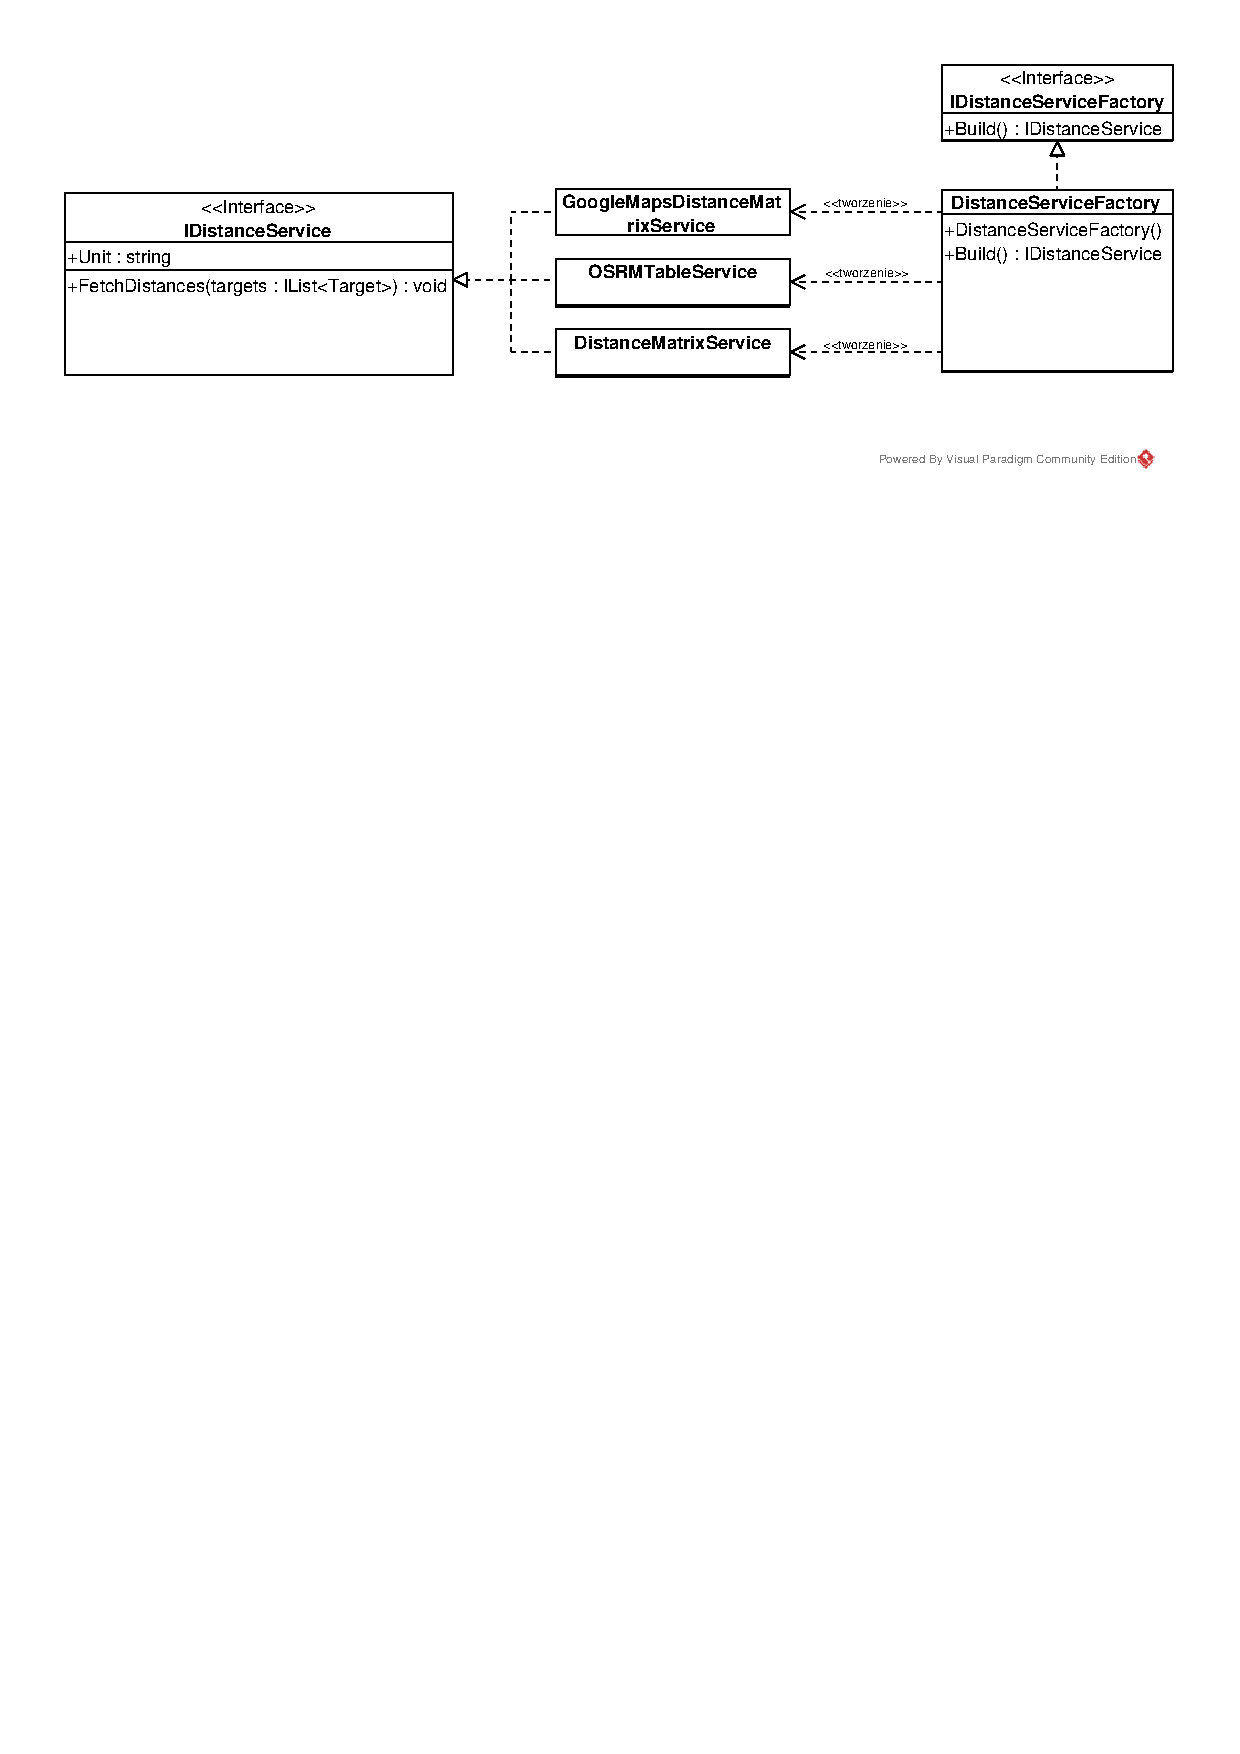
\includegraphics[clip, trim=1cm 23cm 1cm 1cm, width=1.00\textwidth]{uml/fabryka.pdf}
	\caption{Diagram klas fabryki konstruującej klasy pobierające dane zewnętrzne}
	\source{Opracowanie własne na podstawie \cite{wzorce}}
	\label{fig:fabryka}
\end{figure}

\subsection*{MVC}
Wzorzec MVC składa się z trzech typów obiektów: Modelu (\textit{Model}), Widoku (\textit{View}) i Kontrolera (\textit{Controller}). MVC pozwala na oddzielenie widoku użytkownika od warstwy przetwarzania. 

W aplikacji ten wzorzec został użyty do wyświetlenia strony głównej i~ustawień (schemat na rysunku \ref{fig:mvc}). Całym mechanizmem zarządza kontroler \texttt{HomeController}. Dziedziczy po standardowej w ASP.NET klasie abstrakcyjnej \texttt{Controller}. \texttt{HomeController} ma dwie publiczne metody: \texttt{Index()} i \texttt{Settings()}, które służą odpowiednio do wyświetlenia strony głównej oraz podstrony zarządzania konfiguracją. Metody te wywołują konstruktory odpowiednich widoków, które zostały stworzone w HTML z pomocą składni Razor - języka służącego do tworzenia szablonów w ASP.NET.

Kontroler korzysta z modelu opisanego przez interfejs \texttt{IConfigurationService}, który zawiera dwie metody: \texttt{Get()} i \texttt{Save(Configuration config)}. Służy on do pobierania i zapisywania danych konfiguracyjnych. Interfejs ten został zaimplementowany przez klasę \texttt{TargetsFileStorage}. Klasa ta przechowuje zserializowane dane konfiguracyjne na dysku w postaci tekstowego pliku JSON. Kontroler nie tworzy obiektu tej klasy, lecz jest on wstrzykiwany jako zależność. Umożliwia to zamianę implementacji interfejsu na inny, przykładowo korzystający z bazy danych.

\begin{figure}[htbp]
	\centering
	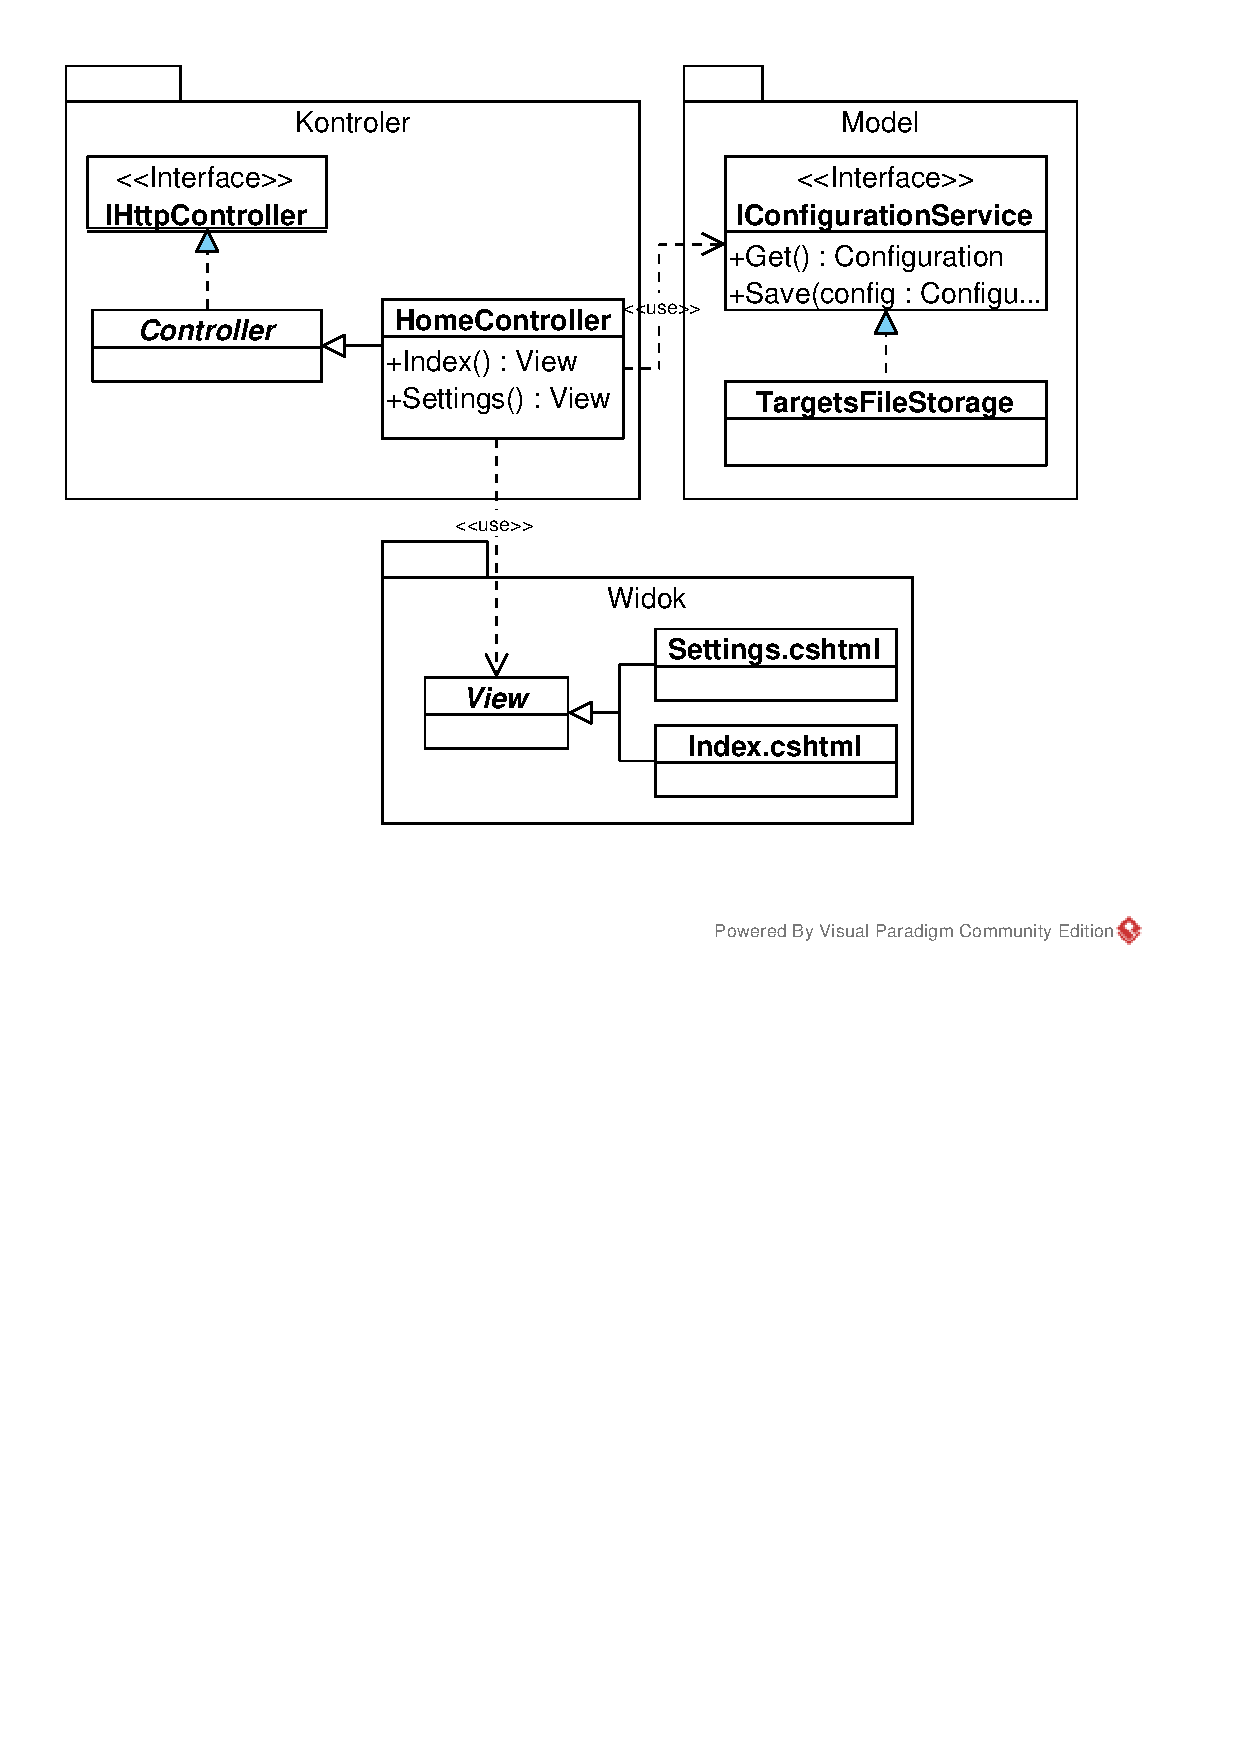
\includegraphics[clip, trim=1cm 15cm 2.5cm 1cm, width=1.00\textwidth]{uml/mvc.pdf}
	\caption{Diagram wzorca MVC w części wyświetlającej strony: główną i ustawień}
	\source{Opracowanie własne}
	\label{fig:mvc}
\end{figure}

\subsection*{Wstrzykiwanie zależności}

Wstrzykiwanie zależności (\textit{Dependency Injection}) jest wzorcem, w którym obiekty wymagane przez klasę do działania są dostarczane przez inny obiekt -- \textit{injector}. Pozwala na usunięcie bezpośredniego powiązania między klasami\cite{wstrzykiwanie}. Dzięki temu klasa korzystająca z zależności nie musi znać implementacji konkretnego obiektu, a operować na interfejsach. Pozwala to na bezproblemową wymianę implementacji na inną.

Klasę przechowującą obiekty i przeprowadzającą wstrzykiwanie nazywa się kontenerem wstrzykiwania zależności (\textit{Dependency Injection Container}). Ponieważ kontener najczęściej zajmuje się stworzeniem obiektów, to w nim konfiguruje się czas ich życia, np. tworzenie instancji na jedno żądanie HTTP lub jedna instancja na całą aplikację (podobnie jak we wzorcu Singleton).

Mechanizm wstrzykiwania jest wspierany w ASP.NET po odpowiedniej konfiguracji. Aplikacja korzysta z gotowego kontenera o nazwie Unity. Pozwala on na wstrzykiwanie zależności do parametrów konstruktora.

Wszystkie kontrolery w opisywanej aplikacji mają zależności wstrzykiwane przez kontener.

\begin{figure}[htbp]
	\centering
	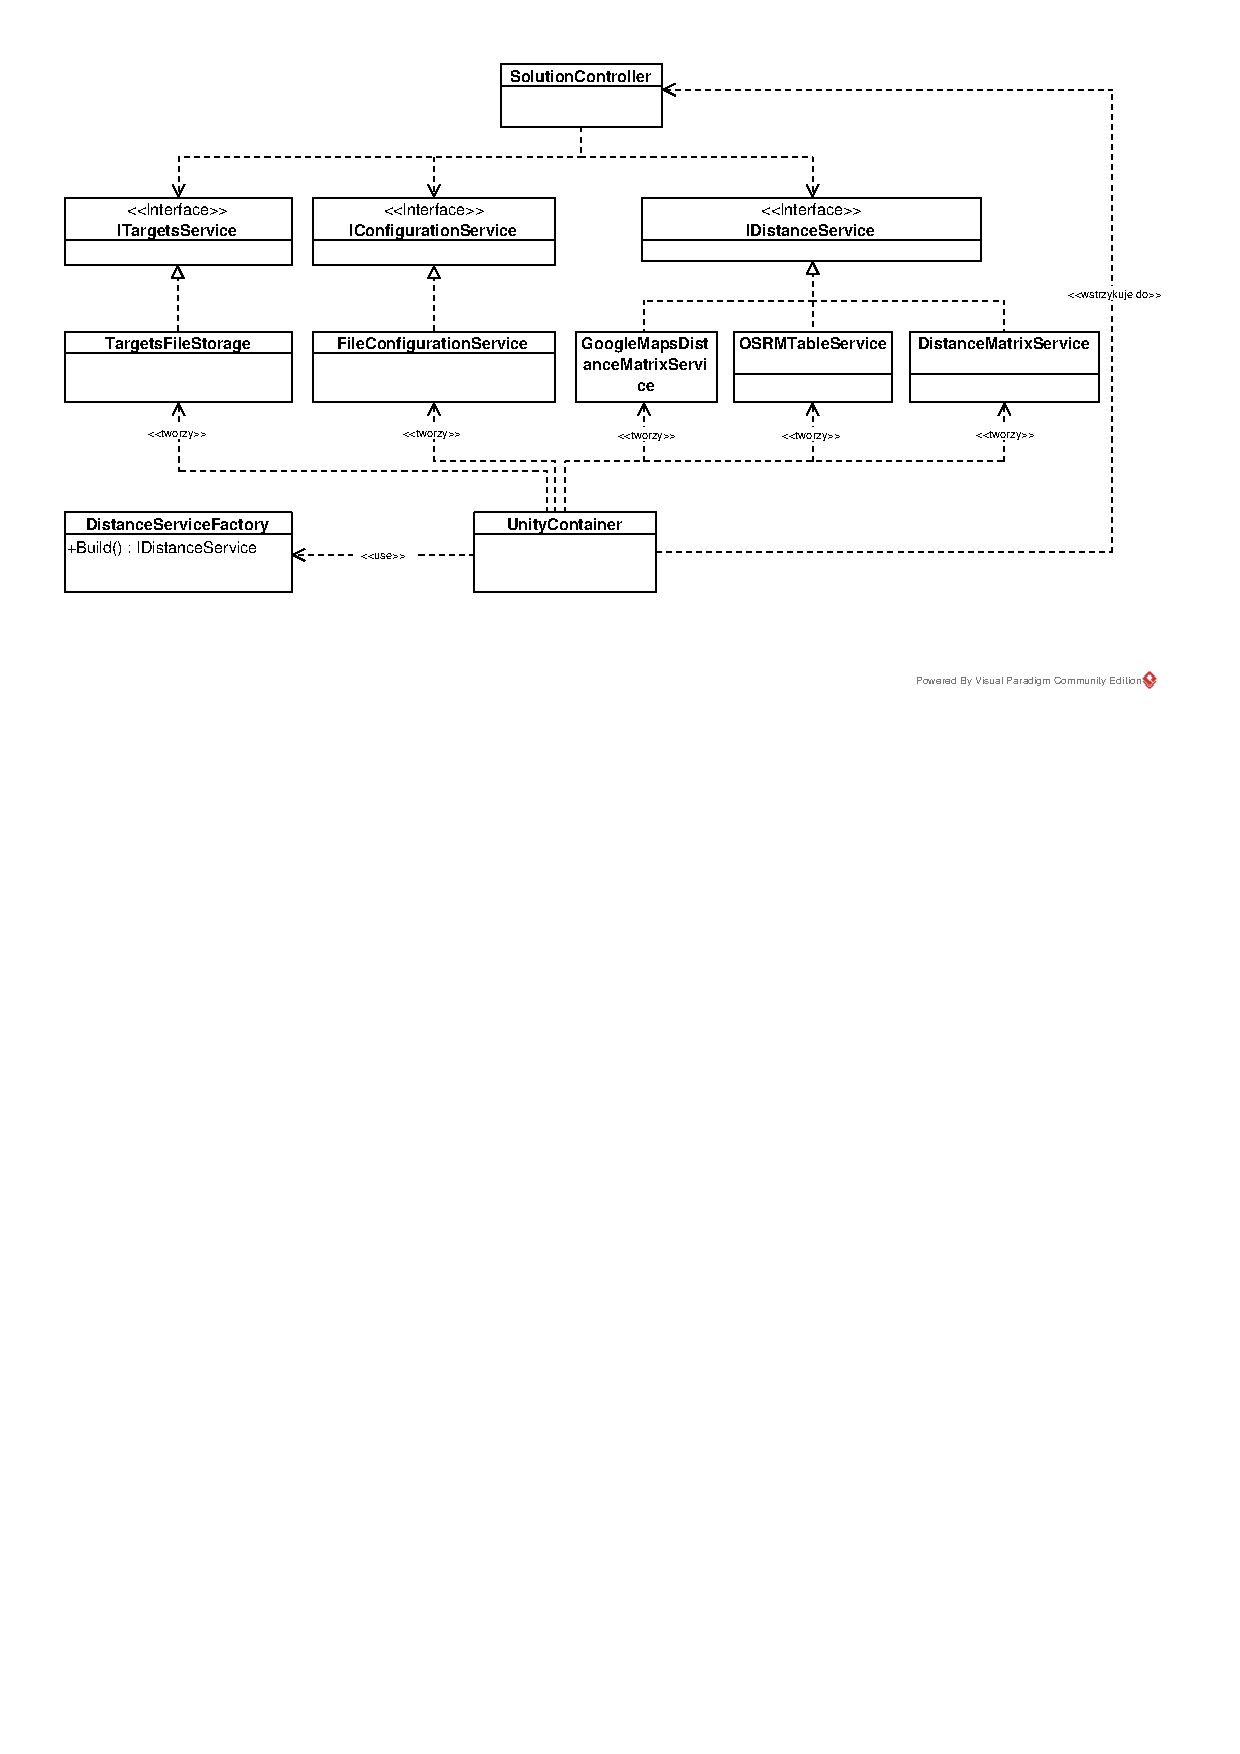
\includegraphics[clip, trim=1cm 19cm 1cm 1cm, width=1.00\textwidth]{uml/injection.pdf}
	\caption{Diagram wstrzykiwania zależności kontrolera}
	\source{Opracowanie własne na podstawie \cite{wstrzykiwanie}}
	\label{fig:di}
\end{figure}

Na rysunku \ref{fig:di} został przedstawiony schemat wstrzykiwania zależności klasy \texttt{SolutionController}. Konstruktor tego kontrolera przyjmuje trzy parametry jako interfejsy. Kontener \texttt{UnityContainer} rozwiązuje zależności wyszukując obiekt implementujący dany interfejs. Ponieważ wszystkim klasom wystarczy jedna instancja na czas działania programu, obiekty zostały uprzednio utworzone przez kontener podczas startu aplikacji.

Klasy implementujące interfejs \texttt{IDistanceService} są tworzone przez wcześniej opisaną fabrykę, natomiast pozostałe zależności są konstruowane bezpośrednio przez kontener.

\clearpage
		\section{Integracja systemów zewnętrznych}
			Ponieważ aplikacja operuje na rzeczywistych mapach, konieczna była integracja z odpowiednimi źródłami danych geograficznych. Program pobiera z systemów zewnętrznych:
\begin{itemize}
	\item odległości między punktami (czas przejazdu lub dystans),
	\item przybliżony adres na podstawie współrzędnych,
	\item graficzne mapy, przeznaczone do wyświetlania.
\end{itemize}

			\subsection{Google Maps}
				Usługa Google Maps udostępnia poprzez API różne usługi za darmo. Konieczna jest rejestracja na stronie firmy Google, gdzie możliwe jest utworzenie klucza identyfikującego aplikację na serwerze. Wygenerowany klucz musi być przesyłany z każdym żądaniem do serwera, w przeciwnym wypadku zostanie odesłana odpowiedź o braku dostępu.

Interfejs Google jest dostępny dla wielu języków i technologii. Program korzysta z dwóch: \textbf{Maps JavaScript API}, działającego po stronie przeglądarki, oraz \textbf{Web Services API}, używanego przez napisany w C\# serwer.

Widoczna na interfejsie użytkownika interaktywna mapa jest utworzona przy pomocy API JavaScript. Umożliwia ono dodanie do strony HTML odpowiedniego widoku graficznego, oraz wykonywanie na nim różnych akcji z poziomu kodu JavaScript, np. zaznaczenia punktów i narysowania odcinków pomiędzy nimi. Możliwa jest także obsługa zdarzeń pochodzących z mapy, np. kliknięcia lub zmiany powiększenia. Tę obsługę realizuje się poprzez tzw. \textit{callbacki}, czyli własne funkcje obsługujące zdarzenie, napisane w JavaScript i~przekazane do obiektów API.

Pozostałe dane są pobierane przez serwer z Web Services API. Jest to przede wszystkim macierz odległości między punktami. \textbf{Google Maps Distance Matrix API} umożliwia wysłanie listy współrzędnych w pojedynczym zapytaniu i otrzymanie odpowiedzi w formacie JSON, zawierającej wszystkie odległości i czasy.

Poważnym ograniczeniem tego API jest wymiar macierzy odległości. Jest to tylko 25 punktów na zapytanie. Ponadto istnieją ograniczenia na dobową i sekundową liczbę zapytań.
			\subsection{OSRM: Open Source Routing Machine}
				Aby móc rozwiązać problem dla większej niż 25 liczby punktów, należy w ustawieniach aplikacji wybrać silnik \textbf{OpenStreetMap}. OpenStreetMap to otwartoźródłowy projekt, mający na celu dostarczyć darmową alternatywę dla map komercyjnych.

Na bazie OpenStreetMap powstał projekt \textbf{OSRM}\footnote{Open Source Routing Machine}. Jest to konsolowy program, możliwy do uruchomienia na własnym komputerze bez dostępu do internetu. Przez udostępnione API HTTP umożliwia m.in. odnajdowanie tras między podanymi współrzędnymi.

Podobnie jak z Google Maps możliwe jest pobranie macierzy w jednym zapytaniu. Zaletą OSRM jest brak ograniczenia liczby punktów (w praktyce ograniczeniem są możliwości komputera na którym uruchomiono program). Niestety zwracana z API macierz zawiera wyłącznie informacje o szacowanych czasach, a nie dystansach. W czasie pisania poniższej pracy nie została ukończona wersja OSRM zwracająca dystanse w macierzy.

W celu skorzystania z OSRM do optymalizacji odległości, aplikacja wysyła wielokrotne zapytania do API - wymaga to wysłania jednego żądania HTTP na jedną odległość. Ponieważ złożoność tego rodzaju pobierania danych to $O(n^{2})$, to jego prędkość jest bardzo wolna. Aby nieco przyspieszyć działanie, aplikacja wysyła zapytania równolegle, z wielu wątków. Jednak ta metoda wciąż pozostaje najwolniejsza - porównanie jej szybkości z innymi znajduje się w rozdziale \ref{sec:wydajnosc}.

Aby uruchomić OSRM lokalnie, można skorzystać z Dockera. Skompilowany projekt jest dostarczony w postaci kontenera, który należy wcześniej skonfigurować. W tym celu trzeba pobrać plik map ze strony OpenStreetMap, następnie udostępnić go Dockerowi i wewnątrz kontenera skompilować go do użycia przez OSRM.

Ponieważ OSRM nie ma potrzeby komunikacji z żadnym zewnętrznym serwisem przez internet, nie ma ograniczeń na liczbę zapytań.
	\chapter{Testowanie aplikacji}
	\section{Testy manualne}
		Aplikacja może być uruchomiona w dowolnej współczesnej przeglądarce. Najważniejszym elementem interfejsu, widocznego na rysunku \ref{screen:1_przed_uruchomieniem} jest mapa. Przesyłki oznaczone są czerwonymi znacznikami, natomiast punkt początkowy zielonym znacznikiem z ikoną ciężarówki.
\begin{figure}[t]
	\centering
	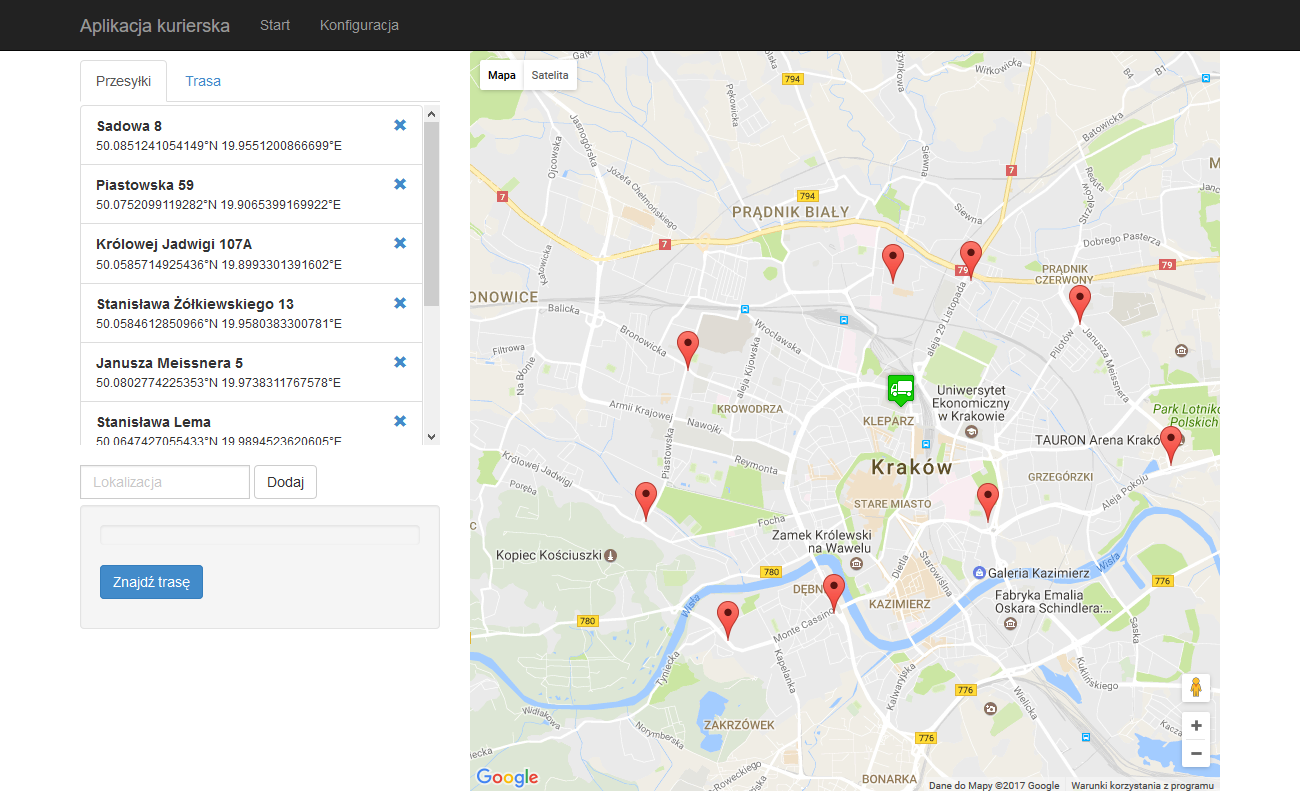
\includegraphics[width=0.7\linewidth]{screen/1_przed_uruchomieniem}
	\caption{Widok aplikacji po dodaniu kilku przesyłek}
	\label{screen:1_przed_uruchomieniem}
\end{figure}

Dodanie przesyłek jest możliwe na dwa sposoby: 
\begin{itemize}
	\item kliknięcie na mapie -- w tym wypadku przybliżony adres zostanie automatycznie znaleziony na podstawie współrzędnych,
	\item wpisanie adresu i naciśnięcie przycisku ,,Dodaj'' -- współrzędne zostaną odnalezione przez wyszukanie adresu.
\end{itemize}

Rezultatem w obu przypadkach jest dodanie przesyłki do listy oraz odpowiedniego punktu na mapie.

Po wprowadzeniu wszystkich punktów, należy nacisnąć przycisk ,,Znajdź trasę''. Uruchamia to proces wyszukiwania trasy na serwerze, a użytkownik widzi w tym czasie animację paska postępu. W przypadku wystąpienia błędu, na przykład z połączeniem, zostanie wyświetlony komunikat z opisem błędu.

Gdy serwer zwróci poprawną odpowiedź (rysunek \ref{screen:2_po_wyszukaniu}), na mapie pokazują się połączenia między punktami trasy. Kolor paska postępu zmienia się na zielony, a poniżej można odczytać łączną długość lub czas potrzebny do przebycia trasy (w zależności od wybranego przez użytkownika sposobu optymalizacji).

\begin{figure}
	\centering
	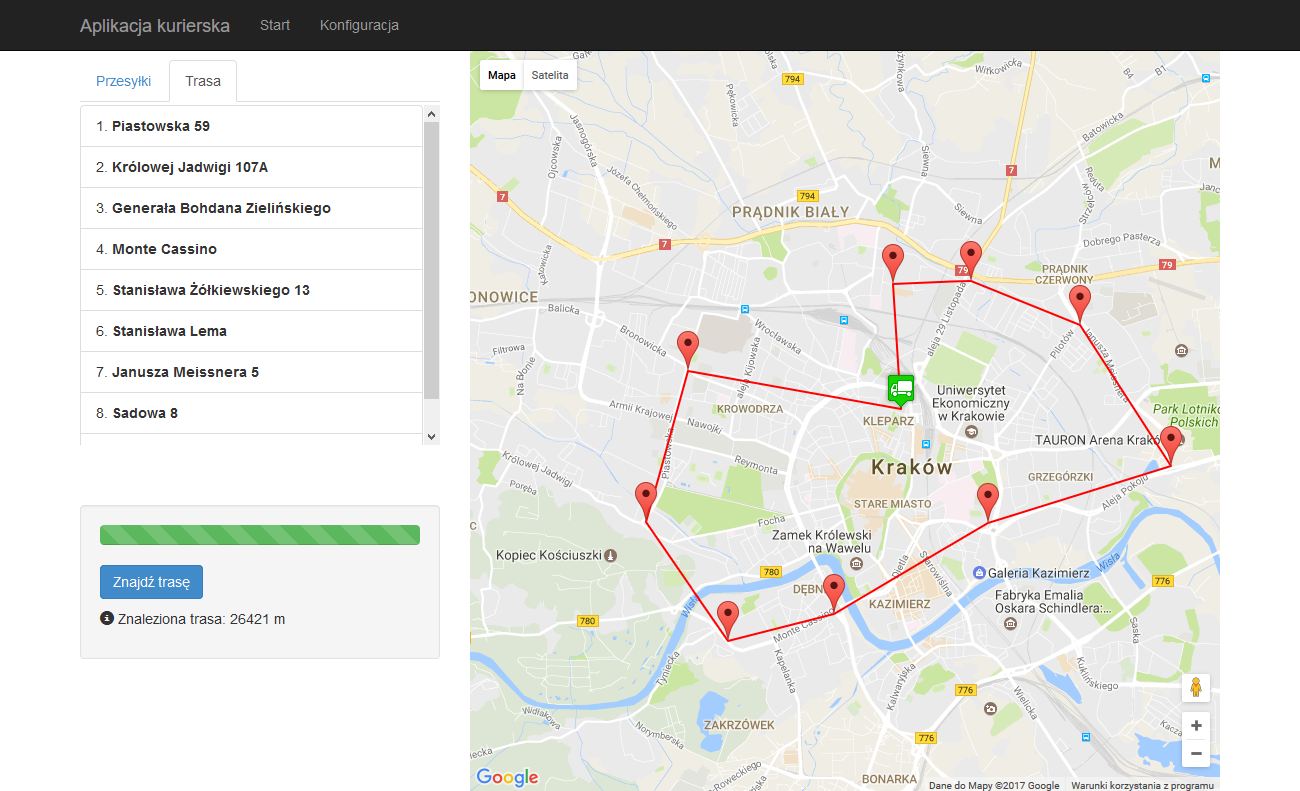
\includegraphics[width=0.7\linewidth]{screen/2_po_wyszukaniu}
	\caption{Mapa z widoczną trasą oraz lista kolejnych celów}
	\label{screen:2_po_wyszukaniu}
\end{figure}

Po wybraniu z menu odnośnika ,,Konfiguracja'' użytkownik ma możliwość zmiany ustawień aplikacji (rysunek \ref{screen:3_konfiguracja}). Okno zostało podzielone na opcje podstawowe, oraz ustawienia silnika przeznaczone dla zaawansowanych użytkowników.

Naciśnięcie przycisku ,,Przywróć domyślne'' resetuje wszystkie ustawienia do stanu początkowego.

Konfiguracja jest zapisywana na dysku serwera w pliku JSON, przez co wartości mogą być odczytane po restarcie serwera.

Do podstawowych opcji należy wybór jednego z trzech rodzajów optymalizacji. Użytkownik ma możliwość wybrania punktu początkowego, czyli siedziby firmy kurierskiej. Wyboru tej lokalizacji dokonuje się poprzez wpisanie adresu lub nazwy miejsca. Aplikacja na bieżąco podpowiada wpisywane adresy.

\begin{figure}
	\centering
	\subcaptionbox{wszystkie dostępne ustawienia\label{screen:3_konfiguracja}}
	{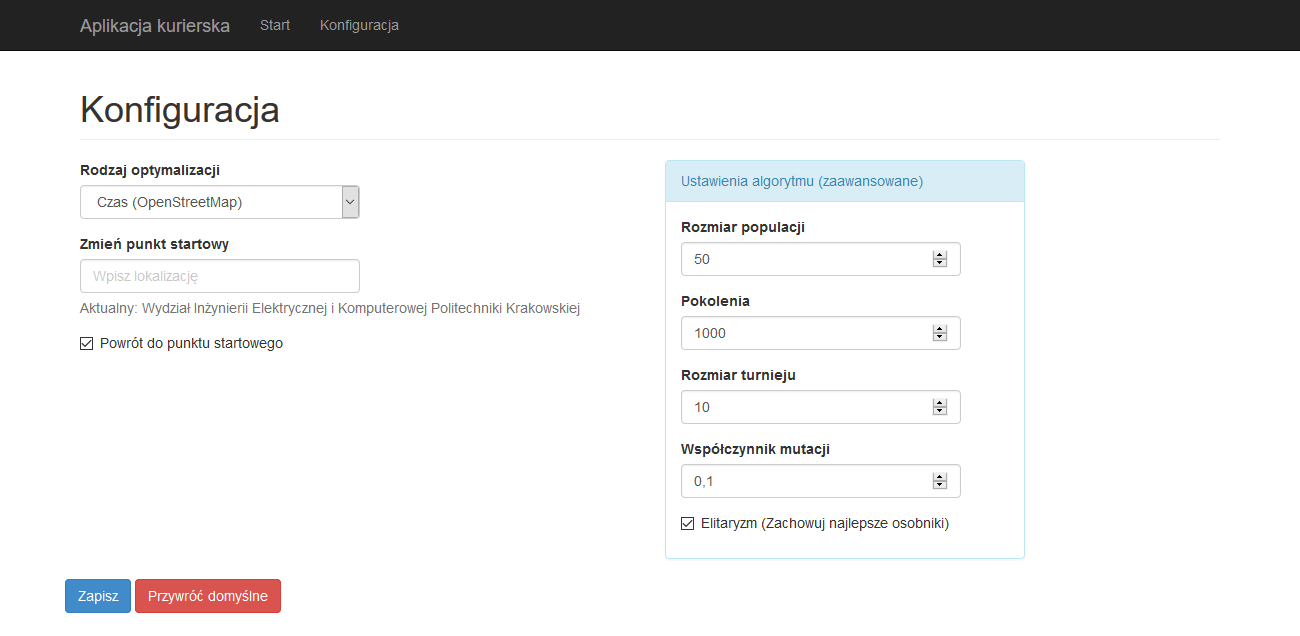
\includegraphics[width=\linewidth]{screen/3_konfiguracja}}
	
	\bigskip
	
	\subcaptionbox{zmiana rodzaju optymalizacji}[0.45\linewidth]
	{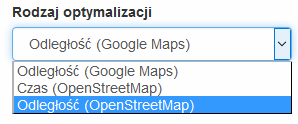
\includegraphics[width=0.4\linewidth]{screen/4a_konfiguracja_cel}}\hfill
	\subcaptionbox{wybór punktu początkowego}[0.45\linewidth]
	{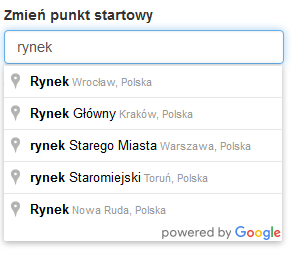
\includegraphics[width=0.4\linewidth]{screen/4b_konfiguracja_start}}
	
	\caption{Ekran konfiguracji}
\end{figure}

\clearpage

W zaawansowanych ustawieniach można dokonać konfiguracji parametrów algorytmu genetycznego. Pozwala to dostosować aplikację do wymagań konkretnego użytkownika, który może preferować większą dokładność optymalizacji lub jej czas.

Odpowiednie dostrojenie parametrów algorytmu umożliwia znalezienie trasy dla większej liczby przesyłek. Na rysunku \ref{screen:5_wiecej_punktow} aplikacja znalazła optymalną trasę dla 30 punktów.

\begin{figure}[H]
	\centering
	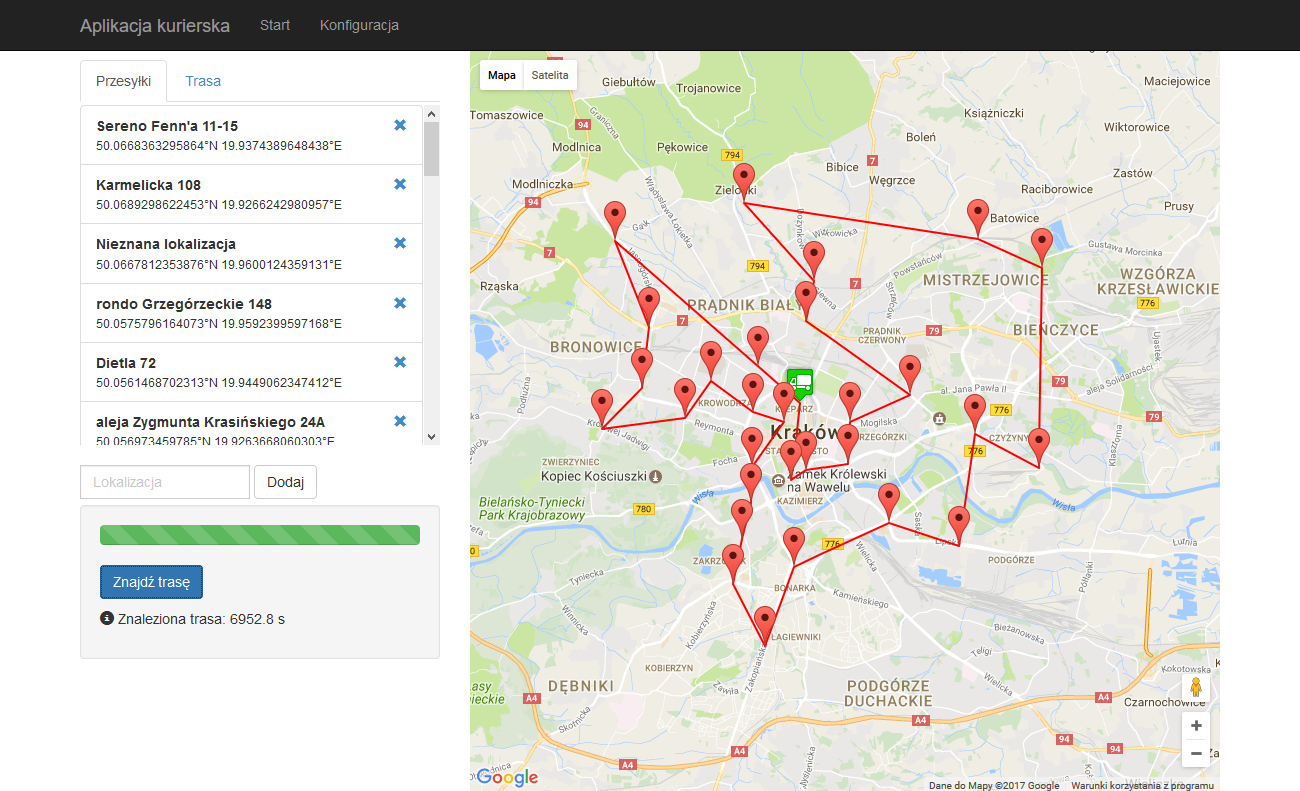
\includegraphics[width=1\linewidth]{screen/5_wiecej_punktow}
	\caption{Znaleziona trasa dla 30 przesyłek}
	\label{screen:5_wiecej_punktow}
\end{figure}

\clearpage
	\section{Testy jednostkowe}
		\label{sec:testy_jednostkowe}
		Projekt zawiera kilka testów jednostkowych, które sprawdzają poprawność poszczególnych komponentów programu. Testy jednostkowe są wykonywane automatycznie, przez co po modyfikacji kodu programu można łatwo upewnić się, czy wprowadzone zmiany są zgodne z testami.

\begin{center}
\begin{forest}
  for tree={
    font=\ttfamily,
    grow'=0,
    child anchor=west,
    parent anchor=south,
    anchor=west,
    calign=first,
    edge path={
      \noexpand\path [draw, \forestoption{edge}]
      (!u.south west) +(7.5pt,0) |- node[fill,inner sep=1.25pt] {} (.child anchor)\forestoption{edge label};
    },
    before typesetting nodes={
      if n=1
        {insert before={[,phantom]}}
        {}
    },
    fit=band,
    before computing xy={l=15pt},
  }
[TSP.Tests
  [SolverTests
	[SimpleProblemTest]
    [ComplexProblemTest]
    [CrossoverDoesntCreateDuplicatesTest]
    [RouteDistanceTest]
  ]
  [TargetTests
    [NorthEastCoordinatesToStringTest]
    [SouthWestCoordinatesToStringTest]
  ]
]
\end{forest}
\end{center}

Dwa testy (\texttt{SimpleProblemTest} i \texttt{ComplexProblemTest}) sprawdzają działanie całego silnika, przy domyślnych ustawieniach. Drugi z testów dostarcza na wejście przykładowy problem przedstawiony we wprowadzeniu.

Test \texttt{CrossoverDoesntCreateDuplicatesTest} gwarantuje że wynik krzyżowania jest poprawny: nie zawiera duplikatów i składa się z tej samej liczby punktów co źródłowe trasy.

\texttt{RouteDistanceTest} zapewnia poprawność obliczania całkowitej długości trasy.

Testy zawarte w klasie \texttt{TargetTests} testują zamianę przykładowych współrzędnych geograficznych na tekst. Jest to istotne, ponieważ w aplikacji występują trzy sposoby zapisu współrzędnych. Ze względu na wykorzystanie dwóch systemów zewnętrznych wymagających różnych formatów, oraz wyświetlanie współrzędnych użytkownikowi, potrzebne są wszystkie trzy:

\begin{itemize}
	\item "$14.123^{\circ}$N $13.345^{\circ}$E" - format przeznaczony do wyświetlania,
	\item "14.123,13.345" - format Google Maps,
	\item "13.345,14.123" - format OSRM.
\end{itemize}



	\section{Badanie wydajności}\label{sec:wydajnosc}
%		Pierwszym etapem poszukiwania rozwiązania jest pobranie danych z serwisu. Aplikacja obsługuje trzy źródła: 
\begin{itemize}
	\item odległości z Google Maps (serwis internetowy, pojedyncze zapytanie),
	\item odległości z OpenStreetMap (serwis lokalny, wiele zapytań równoległych)
	\item czas przejazdu z OpenStreetMap (serwis lokalny, pojedyncze zapytanie) 
\end{itemize}

Wyniki pomiarów wydajności dla 10 punktów zostały przedstawione w tabeli \ref{tab:pobieranie} oraz na wykresie \ref{chart:pobieranie}.

\begin{table}[t!]
	\centering
	\caption{Czas pobierania danych dla różnych metod [ms]}
	\label{tab:pobieranie}
	\begin{tabular}{r|ccc}
& \textbf{Google Maps} & \textbf{\begin{tabular}[c]{@{}c@{}}OSRM \\ (dystans)\end{tabular}} & \textbf{\begin{tabular}[c]{@{}c@{}}OSRM \\ (czas)\end{tabular}} \\ \hline
& 601                  & 7797                                                               & 62                                                                 \\
& 447                  & 1074                                                               & 31                                                                 \\
& 446                  & 6747                                                               & 26                                                                 \\
& 454                  & 1046                                                               & 45                                                                 \\
& 423                  & 1228                                                               & 34                                                                 \\
& 437                  & 7176                                                               & 29                                                                 \\
& 492                  & 960                                                                & 21                                                                 \\
& 948                  & 1073                                                               & 40                                                                 \\
& 472                  & 6859                                                               & 19                                                                 \\
& 415                  & 7379                                                               & 30                                                                 \\ \hline
\textbf{Średnia} & \textbf{513.5}       & \textbf{4133.9}                                                    & \textbf{33.7}                                                      \\ \hline
Maksimum         & 948                  & 7797                                                               & 62                                                                 \\ \hline
Minimum          & 415                  & 960                                                                & 19                                                                

	\end{tabular}
	\source{Opracowanie własne}
\end{table}
\begin{figure}[b!]
	\caption{Czas pobierania danych dla różnych metod: wykres}
	\begin{bchart}[max=5000, step=1000, unit=ms]
		\label{chart:pobieranie}
		\bcbar[label=Google Maps]{513.5}
		\smallskip
		\bcbar[label=OSRM (dystans)]{4133.9}
		\smallskip
		\bcbar[label=OSRM (czas)]{33.7}
	\end{bchart}
	\source{Opracowanie własne}
\end{figure}

\clearpage
Po wykonaniu powyższych pomiarów okazało się że najszybszą metodą jest pobieranie macierzy czasów przejazdów z lokalnego serwisu OSRM. Jest to zgodne z przewidywaniami, gdyż cała macierz jest pobierana w jednym zapytaniu HTTP oraz nie występują opóźnienia spowodowane transmisją sieciową.
	\chapter*{Podsumowanie}
		\addcontentsline{toc}{chapter}{Podsumowanie}
		Efektem niniejszej pracy jest działająca aplikacja, realizująca zgodnie z założeniami postawione zadanie jakim jest odnajdowanie optymalnych tras dla problemu komiwojażera. Program może być wykorzystywany przez kurierów, listonoszy ale też inne osoby, których praca wymaga szybkiego poruszania się po obszarze miasta, na przykład przedstawicieli handlowych, pośredników nieruchomości.

Wybór algorytmu genetycznego pozwolił na osiągnięcie odpowiedniej optymalizacji odnajdowanych tras, mimo że należy do algorytmów przybliżonych. 

Aplikacja może być łatwo rozwijana w przyszłości. Język C\#, w jakim powstał kod umożliwia integrację z C++, co pozwala na uzyskanie jeszcze lepszej wydajności (przy zachowaniu pełnej funkcjonalności) po przepisaniu części obliczeniowej na język kompilowany do kodu natywnego.
Dzięki oparciu API o standard HTTP możliwe jest łatwe stworzenie dodatkowych interfejsów użytkownika, w formie aplikacji mobilnej lub okienkowej.
Elastyczna konstrukcja silnika, zbudowanego z użyciem wzorców projektowych pozwala na dodanie i rozbudowę jego poszczególnych części, takich jak algorytmy krzyżowania i~selekcji lub całkowitą zamianę typu algorytmu na inny niż genetyczny.
	\bibliographystyle{plain}
	\bibliography{bibliografia}
	\addcontentsline{toc}{chapter}{Bibliografia}
\end{document}